\section{Foundations of Efficiency}
Understanding the fundamental energy demands of a vehicle requires a return to first principles. This section lays the groundwork for quantifying how physical forces, design parameters, and user behavior interact to determine the real-world efficiency of small personal vehicles. Starting from the classical longitudinal force balance, we derive expressions for cruising power and highlight the dominant energy losses during motion. However, idealized conditions rarely hold in practice. Therefore, we extend the model to consider dynamic driving modes—such as idling, acceleration, and braking—as well as the energy implications of vehicle mass and manufacturing. By identifying and isolating these different contributors, we clarify which design decisions offer the greatest potential for reducing energy use, both in operation and over the vehicle’s full lifecycle.
\subsection{Longitudinal Dynamics: A First-Principles Approach}
The force acting longitudinally on a vehicle can be modeled by the following : 

\begin{figure}[h!]
    \centering
    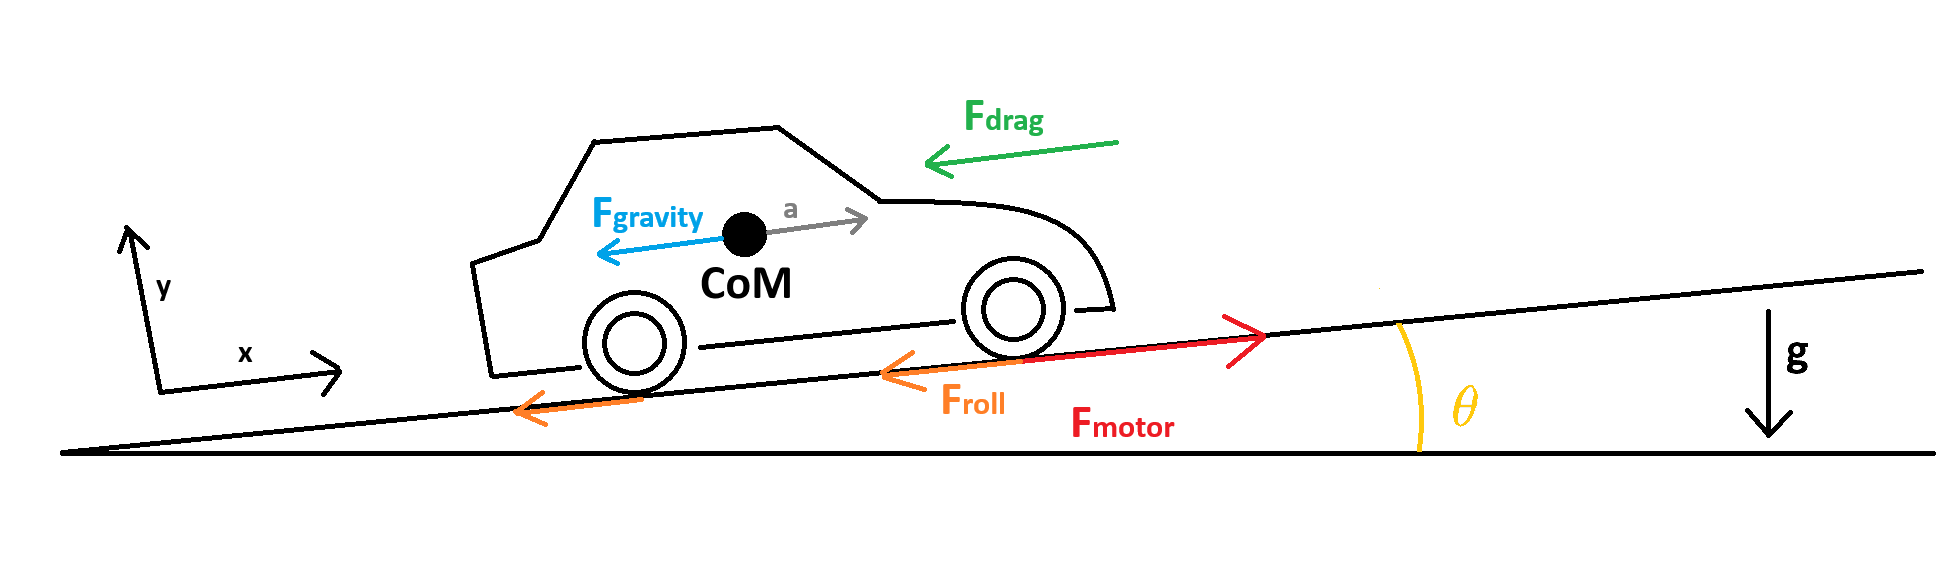
\includegraphics[width=1\linewidth]{Figures/ch1_ForceAxis.png}
    \caption{Longitudinal car dynamics}
    \label{fig:longcardynamics}
\end{figure}

\[
m\cdot a = F_{\text{motor}} - F_{\text{drag}} - F_{\text{roll}} + F_{\text{gravity}}
\]
where:
\begin{itemize}
    \item \textbf{Aerodynamic Drag:} 
    \[
    F_{\text{drag}} = \frac{1}{2} \rho\, C_d\, A\, v^2,
    \]
    with \(\rho\) being the air density, \(C_d\) the drag coefficient, \(A\) the frontal area, and \(v\) the vehicle speed.
    \item \textbf{Rolling Resistance:} 
    \[
    F_{\text{roll}} = C_{rr}\, m\, g,
    \]
    where \(C_{rr}\) is the rolling resistance coefficient, \(m\) the vehicle mass, and \(g\) the gravitational acceleration.
    \item \textbf{Gravitational Component:} 
    \[
    F_{\text{gravity}} = m\, g\, \sin\theta,
    \]
    representing the component of gravity along the road when the vehicle is on an slope with angle \(\theta\). this term become positive when we go downhill, the slope's angle $\theta$ is defined as negative downhill and positive uphill. for a round trip, the gravity term should cancel out. But not the losses from storing and restoring the energy through the power train.
    \item \textbf{Force from motor Acceleration/Braking} 
    \[
    F_{\text{motor}}
    \]
    this term model the force by the motor/brake
\end{itemize}

Energy can be defined as a force endured over a distance. Similarly, power can be defined as a force endured at a given speed. Energy efficiency in this context can be defined by the amount of energy required to move by a given distance. This can be brought back to a force.\\

Vehicle Energy efficiency (cruising), measured as force as a function of speed (the others parameters usually remain nearly constant while travelling)

\begin{equation}
\eta(v) = \cdot\left( \frac{1}{2}\,\rho\,C_d\,A\,v^2 + C_{rr}\,m\,g\right) \quad \text{[N]}.
\label{eq:energy_consumption}
\end{equation}


This gives an idea of what we can tune to minimize the amount of energy per unit of distance. Naturally, this model simplifies the reality by ignoring the energy wasted due to the acceleration/braking/idling cycle due to, e.g., a red light or the increased drag from wind. It also ignores the embodied energy in the vehicle and the power train efficiency.

\subsection{Driving Patterns: Beyond Idealized Model}

To model more accurately the efficiency of a vehicle, we must factor the different driving condition and their relative weight over an average trip. A car can typically be modelled with four distinct driving mode : Cruising, accelerating, braking and idling. There is a fair amount of research studying theses driving modes and their relative proportion. Even tho the exact proportion of each phase is subject to variation, we can nonetheless see that no phase can be neglected, and thus we need to have a vehicle that is efficient in each case.

\begin{figure}[h!]
    \centering
    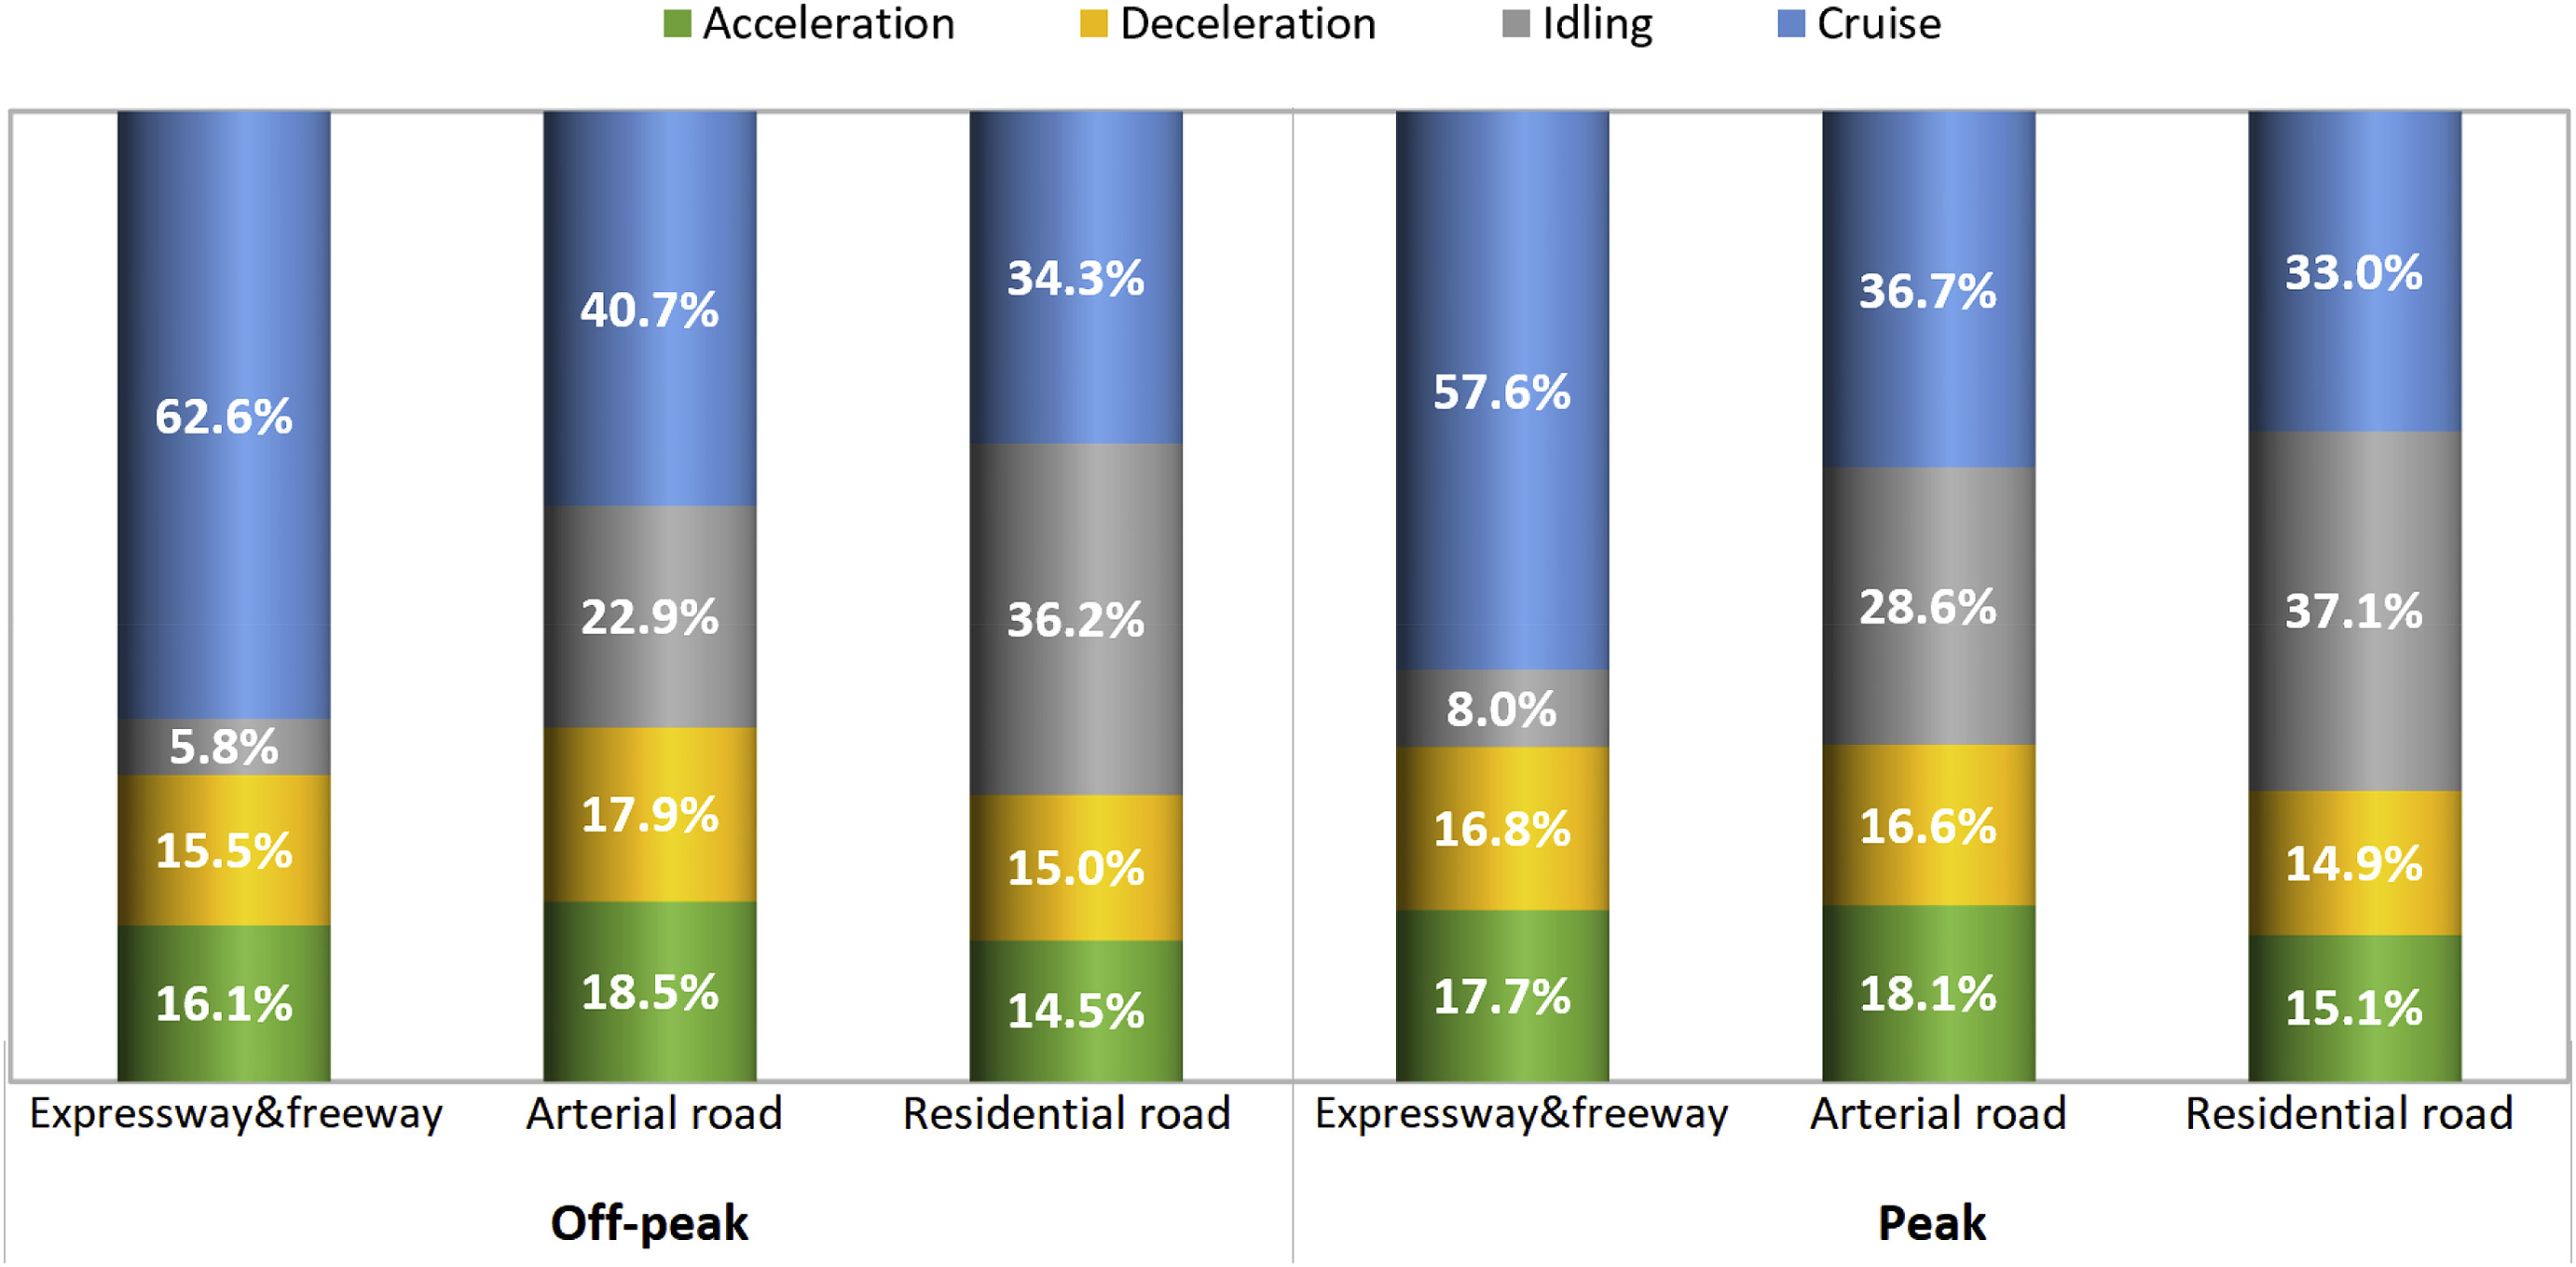
\includegraphics[width=0.8\linewidth]{Figures/ch2_shareOfDrivingModeChina.jpg}
    \caption{Figure from Ma, Real-World driving cycle\cite{ma_real-world_2019} measuring the relative proportion of driving mode}
    \label{fig:ch2proportiondrivingmode}
\end{figure}

We can also notice that the majority of trips are fairly short in Europe, with 80\% being less than 10 [km] and 22 [minutes], warm-up time must be taken into account if required as it's the case for internal combustion engine. The trips being fairly short, it's reasonable to assume that the driver could sustain an effort during this time frame if the power at play is comparable to what a human being can output.

\begin{figure}[h!]
    \centering
    \subfloat{
        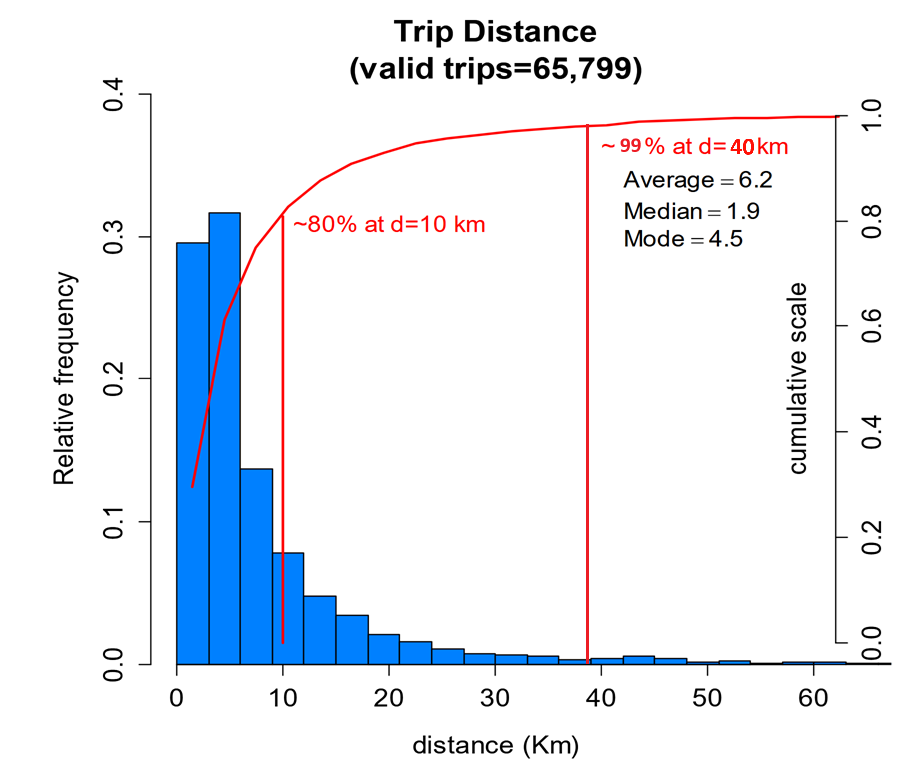
\includegraphics[width=0.45\linewidth]{Figures/ch2_TripsLenghtFrequency.png}
        \label{fig:trips-length}
    }
    \hfill
    \subfloat{
        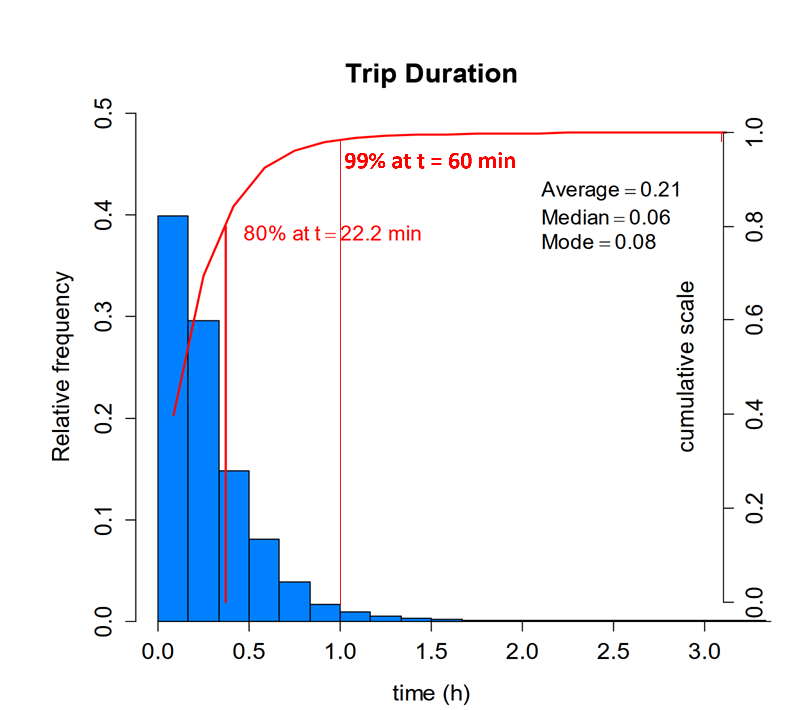
\includegraphics[width=0.45\linewidth]{Figures/ch2_TripsDurationFrequency.png}
        \label{fig:trips-duration}
    }
    \caption{Comparison of trip length and trip duration frequency distributions. Relative frequency (bar) and cumulative (red, solid) (from Donati 2015\cite{donati_individual_2015})}
    \label{fig:trips-comparison}
\end{figure}

we can define an idling efficiency (even tho the vehicle is not moving and thus only wasting energy, some will waste more energy per unit of time than others)

we can define a deceleration efficiency, measuring how much energy we can recover while braking (0\% for a typical ICE vehicle up to 70\% for an electric vehicle with regenerative braking \cite{noauthor_regenerative_nodate}). This figure is useful both to describe regenerative breaking while going downhill or in a deceleration scenario.

we can define an acceleration efficiency by looking at how much energy is wasted from the tank/battery to the wheel/kinetic energy, with value as low as 13\% between and the tank and the wheel for an ICE car and up to 80\% for an electric car \cite{lohse-busch_ambient_2013}. This figure is useful to describe both scenario where the vehicle is climbing a hill and scenario where the vehicle is accelerating.

\subsection{Embodied Energy and Material Impact: Why Mass Matters }

while this work will not go too deep into the manufacturing impact of the vehicle, it's important to note that a significant amount of resources is used and that electric vehicle tend to be more energy and resources intensive than ICE vehicle during its manufacturing, but ICE vehicle compensate by a higher energy and emissions during its life. As the power grid get less carbon intensive, manufacturing become the limiting factor. To reduce the impact of the manufacturing, the vehicle should last as long as possible and minimize the mass of energy intensive material.

\begin{table}[h]
    \centering
    \begin{tabular}{lccc}
        \toprule
        \textbf{Vehicle} & \textbf{Lifecycle} & \textbf{Emissions} \\
        \textbf{Type} & \textbf{Emissions} & \textbf{in Prod.} \\
        & \textbf{(tonnes CO2e)} & \textbf{(tonnes CO2e)} \\
        \midrule
        Standard gasoline vehicle & 24  & 5.6 \\
        Hybrid vehicle            & 21  & 6.5 \\
        Plug-in hybrid vehicle    & 19  & 6.7 \\
        Battery electric vehicle (~500 [g/kWh] CO2e)  & 19  & 8.8 \\
        Battery electric vehicle (~100 [g/kWh] CO2e)  & 10.8 & 8.8 \\
        \bottomrule
    \end{tabular}
    \caption{Vehicle Whole Life Carbon Emissions Analysis, based upon a 2015 vehicle in use for 150'000 [Km] using 10\% ethanol blend. Data from \cite{noauthor_zemo2025lifecycle_nodate}, the energy intensity of the power grid correspond to the world (500g/kWh) and Europe (100g/kWh) average respectively, some country doing way better and other worse.\cite{noauthor_power_nodate}}
    \label{tab:carbon_emissions}
\end{table}

\newpage

\subsection{Parameters affecting Efficiency}

From the previous equations \eqref{eq:energy_consumption}, we see that to improve the efficiency we must minimize the mass $m$ and frontal area $A$ of the vehicle followed by a reduction of $C_d$ and $C_{rr}$. Furthermore, the power train efficiency is quite important as braking and acceleration cycle are frequent and thus energy is lost every time energy is converted back and forth. Finally, we must also maximize the idling efficiency, as the vehicle will spend a non-negligible amount of time stopped.


\subsection{Aerodynamic Optimization Through Form Factor}

Designing a narrow and short vehicle naturally limits the frontal area $A$. To further improve $C_d A$, the rider or passenger can be reclined and positioned in tandem configuration. The challenge here is comfort and user experience.

External sensors and digital displays could theoretically solve the visibility issue if one want to further reduce the frontal area, but the resulting cognitive dissonance (visual/vestibular mismatch) can lead to motion sickness. A pragmatic compromise includes a partially reclined posture with sufficient external visibility.

\begin{figure}[h!]
    \centering
    \subfloat{
        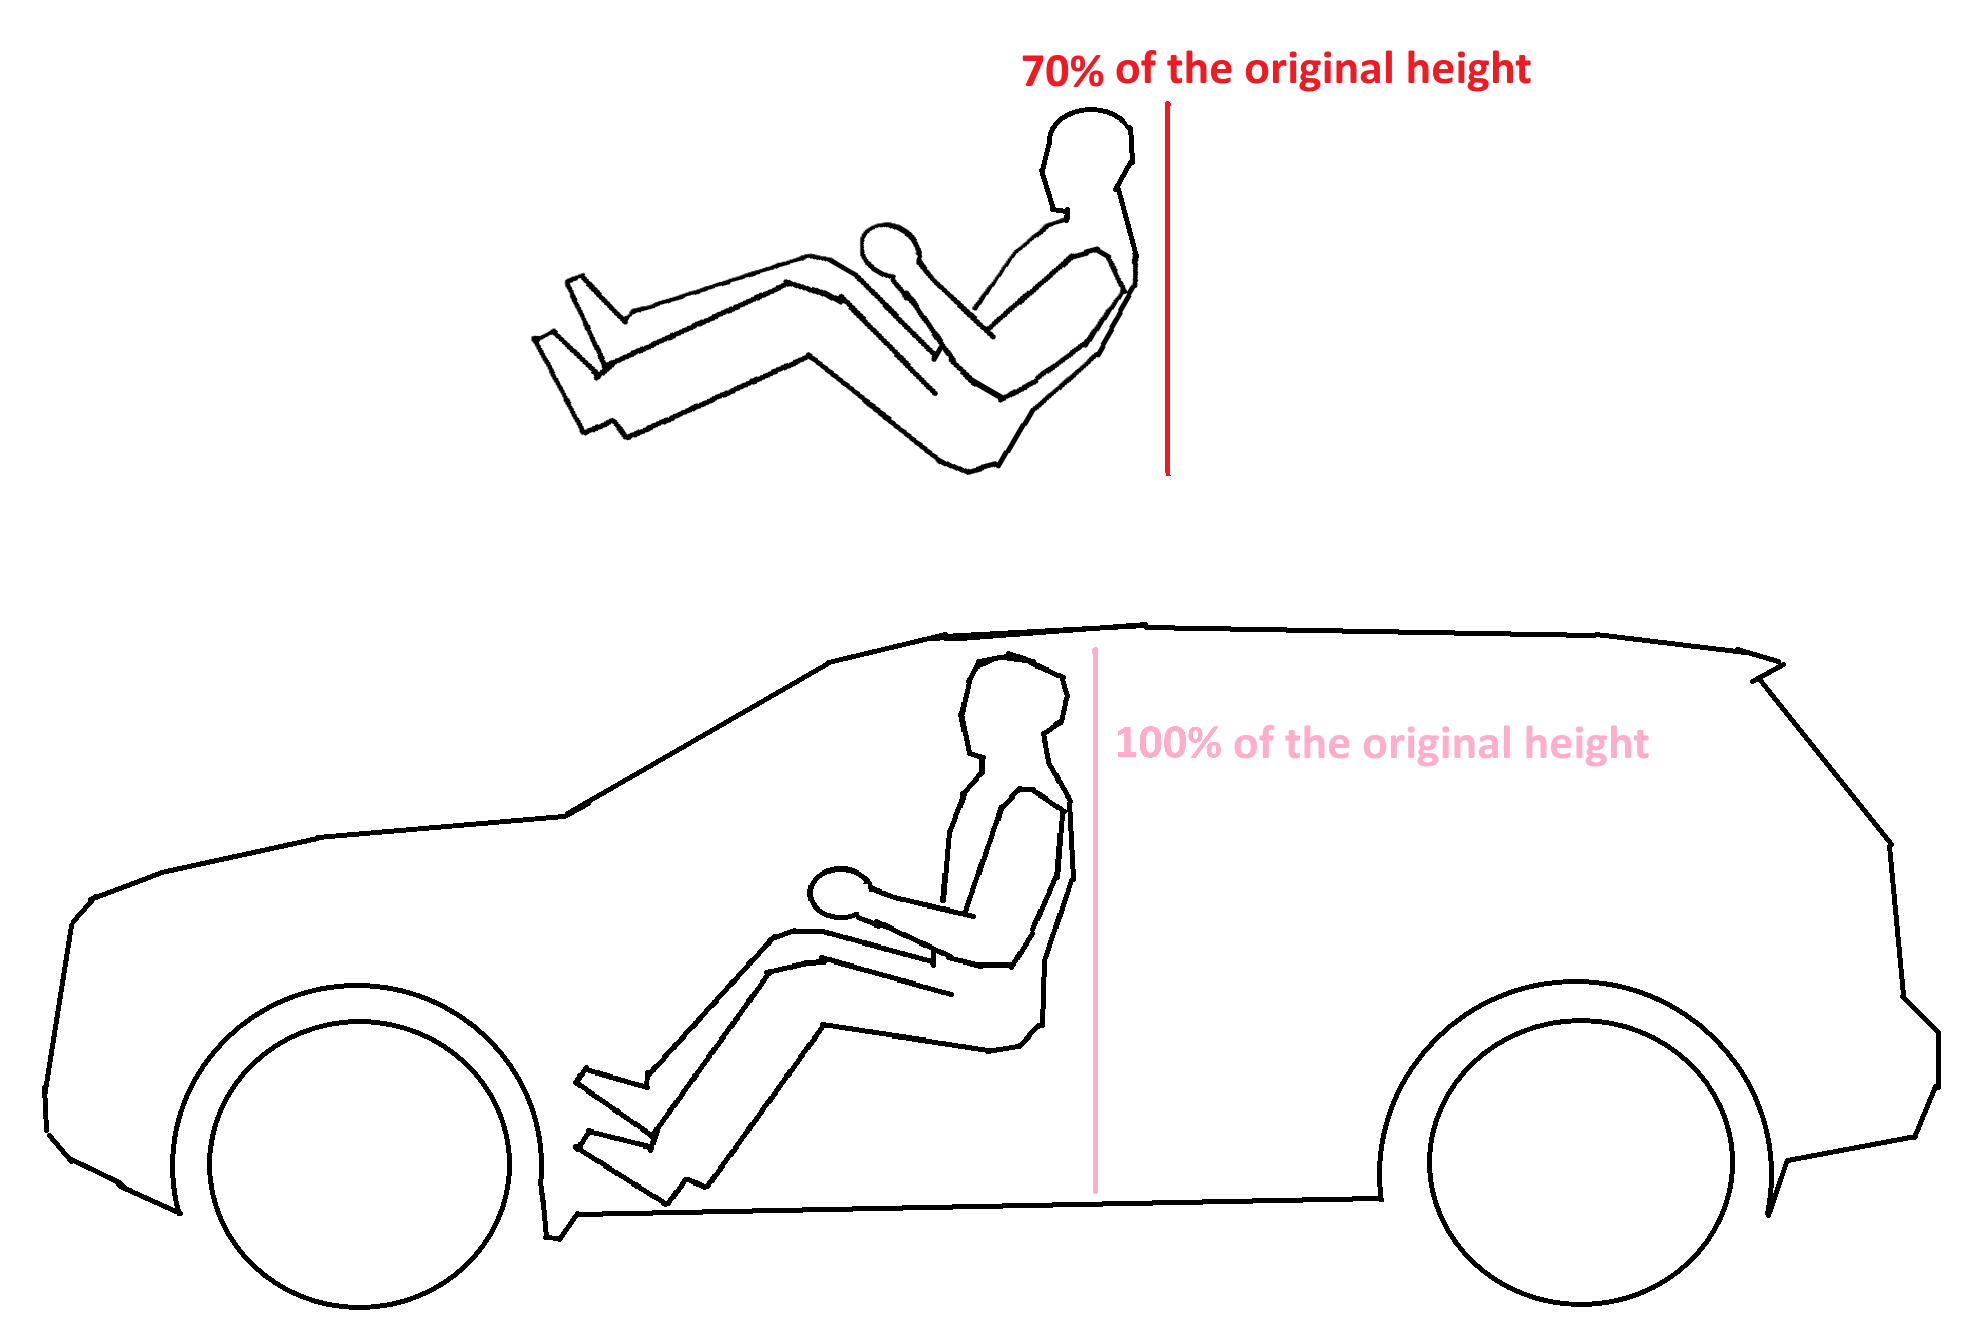
\includegraphics[width=0.47\linewidth]{Figures/ch3_seatingOptimisation.png}
    }
    \hfill
    \subfloat{
        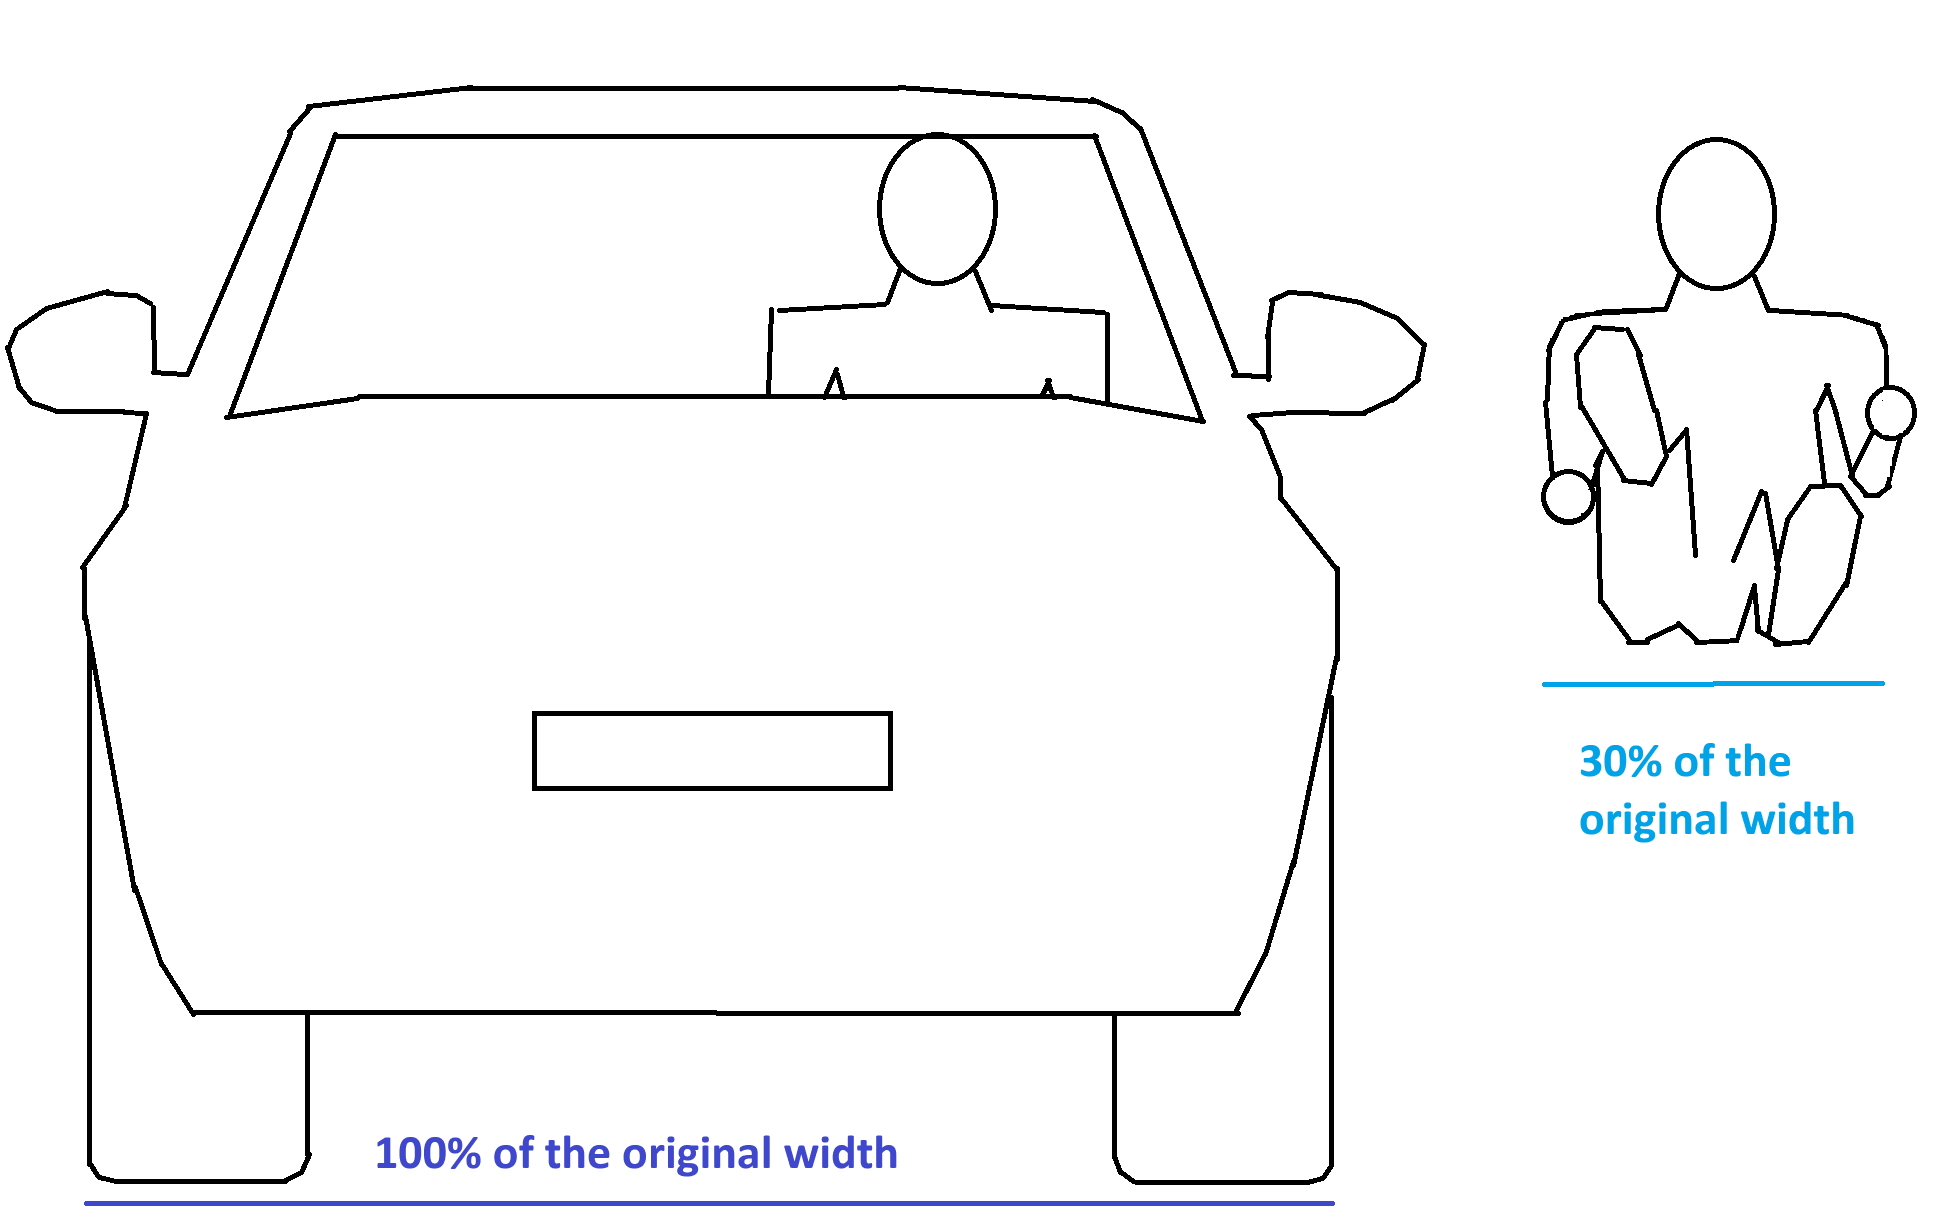
\includegraphics[width=0.47\linewidth]{Figures/ch3_seatingOptimisationFront.png}
    }
    \caption{Effect on the frontal area by reclining the seat by 30° and placing passengers in tandem}
    \label{fig:FrontaAreaGraphicsComparison}
\end{figure}

\newpage 

\begin{figure}[h!]
    \centering
    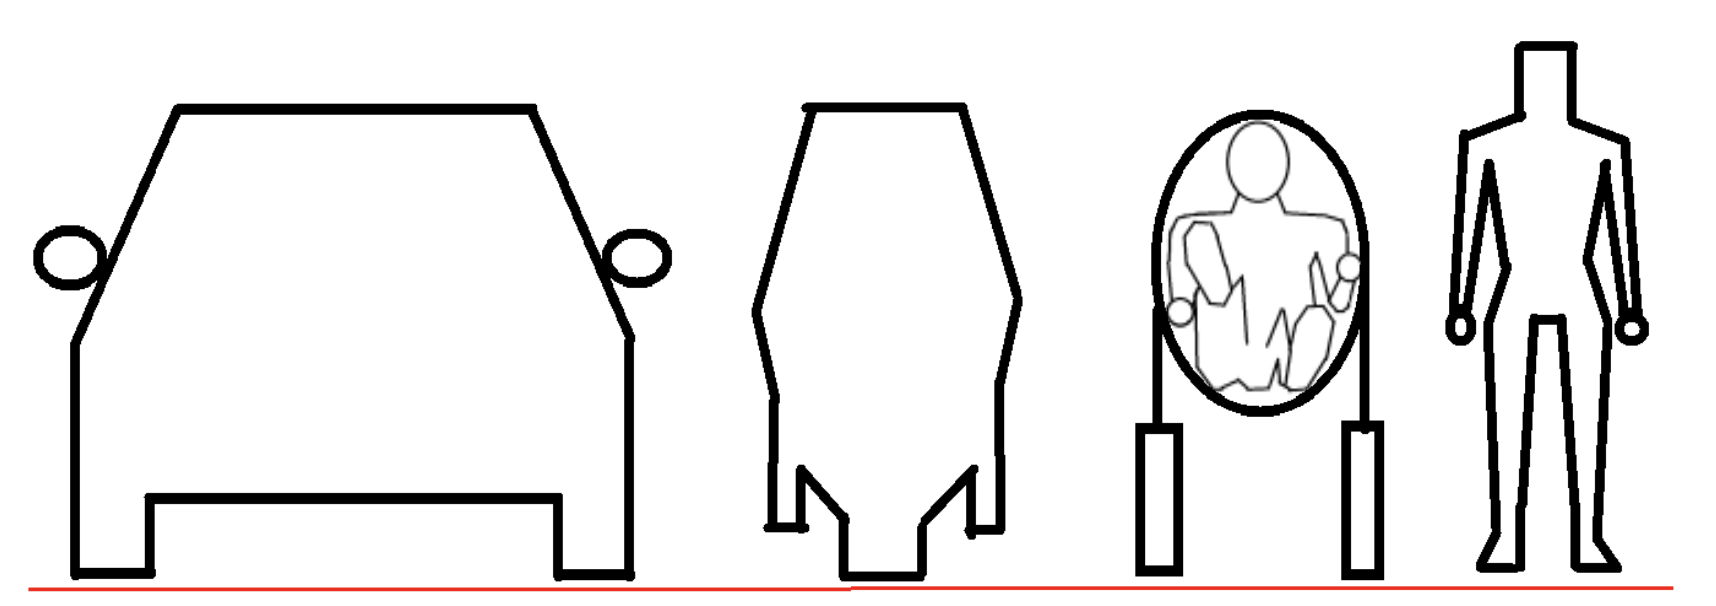
\includegraphics[width=1\linewidth]{Figures/ch4_frontComparisonVehicle.png}
    \caption{Comparison of the frontal area of a car, a leaning vehicle, the proposed solution and a person}
    \label{fig:frontal_comparison}
\end{figure}

But, such configurations, while aerodynamic, make it hard to enter/exit for the passenger. Our design proposes the use of an active system that can adjust the height of each wheel to both solve the leaning during turn problem and allow reclining the seat for easier ingress and egress, solving both problems.

